\documentclass[11pt]{article}

%packages
\usepackage{mathtools}
\usepackage{amsmath}
\usepackage{amssymb}
\usepackage{listings}
\usepackage{xcolor}
\usepackage{graphicx}
\usepackage[margin=1in]{geometry}

%Is this metadata? Title writing info
\title{Enzyme Kinetics in R}
\author{Zane Billings}
\date{}

%Define commands
\newcommand{\np}{\vfill\newpage}
\newcommand{\R}{\texttt{R}}

%Defined colors for xcolor package
\definecolor{cp}{HTML}{592C88} %cp = catamount purple
\definecolor{cg}{HTML}{C1A875} %cg = catamount gold

%Define lstlisting environment appaerance
\lstset{language=R,numbers=left,frame=shadowbox, rulesepcolor=\color{cp}, rulecolor=\color{cg}}

\begin{document}

\maketitle

\section*{Background}
\subsection*{What is Enzyme Kinetics?}
Enzyme kinetics is a subfield of biochemistry which studies the dynamics of chemical reactions which are catalyzed by {\bf enzymes}. Enzymes are a specialized class of protein molecule that have special properties allowing them to speed up biological reactions: this is called the catalytic function of an enzyme.

Enzyme kinetics experiments usually involve taking a known amount of an enzyme, adding it to several different concentrations of its {\bf substrate} (the molecule that the enzyme can interact with), and using an analytical laboratory technique in order to analyze the velocity of the enzyme. Several methods exist for measuring enzyme velocities during a reaction, but the most common are spectrophotometry, radiometry, and fluorescence methods.

\subsection*{Michaelis-Menten Kinetics}
The easiest type of enzymes to describe mathematically are the class of enzymes which are said to follow {\bf Michaelis-Menten kinetics}. Leoner Michaelis and Maud Menten were two biochemists who gave the mathematical model for these enzymes in the beginning of the twentieth century.

In order for an enzyme to fit this model, we must make a few {\bf assumptions}.
\begin{itemize}
	\item All of the enzyme and substrate molecules can diffuse freely (i.e. move wherever they want without constraints) in their container.
	\item The enzyme only binds to one substrate. Enzymes which bind to multiple different substrates (often at the same time) become more complicated and the derivation of their kinematic equations is much more difficult.
	\item The rate of reaction of the enzyme is only affected by two things: intrinsic chemical properties of the enzyme, and the concentration of the substrate. The enzyme can work faster with more substrate, up until the ``saturation point'', where all available enzymes are filled with substrate and the rate of the reaction is capped.
	\item The concentration of the enzyme is much lower than that of the substrate.
\end{itemize}

If we meet all of these conditions, we can describe the rate of the enzyme-substrate reaction with the {\bf Michaelis-Menten Equation}.
\[
V = \frac{v_{\mathrm{max}}[S]}{K_m + [S]}
\]
In the equation, \(V\) is the reaction rate, \(v_{\mathrm{max}}\) is the maximum possible reaction rate, \(K_m\) is the Michaelis-Menten constant, a unique property of every enzyme which describes the concentration of the substrate required for the velocity to reach one half of \(v_{\mathrm{max}}\), and \([S]\) is the concentration of the substrate.

\np

\section*{The Lineweaver-Burk Plot}

Lineweaver and Burk were two biochemists who studied enzyme kinetics and developed a method for using least-squares linear regression to estimate the values of \(K_m\) and \(v_{\mathrm{max}}\) from kinetics data. The LB-plot is also known as a {\bf double-reciprocal plot}. 

Suppose we are testing an enzyme that we will call Hoopsase (almost all enzyme names end with the suffix ``-ase''). We have done a lot of spectrophotometry over the last few days, and we have collected the following data set.

\begin{table}[h!]
\centering
\begin{tabular}{c|c}
	[S], \(\mu\)M & Velocity \(\mu\)Ms\(^{-1}\) \\
	\hline
	2 & 2.9 \\
	3 & 3.8 \\
	4 & 4.4 \\
	5 & 5.0 \\
	6 & 5.4 \\
	7 & 5.8 \\
	8 & 6.2 \\
	9 & 6.4 \\
	10 & 6.7 
\end{tabular}
\caption{Velocity data for various substrate concentrations of the enzyme Hoopsase.}
\label{t:Hoopsase}
\end{table}

You may use the following code snippet to create a data frame with this information in \R. (Change ``ex'' to whatever you want the name to be, of course. I recommend changing the column names as it will be less confusing in the long run.)
\begin{lstlisting}
ex <- data.frame(matrix(c(2,3,4,5,6,7,8,9,10,
                   2.9,3.8,4.4,5.0,5.4,5.8,6.2,6.4,6.7),
                 ncol = 2, byrow = FALSE))
colnames(ex) <- c("S","V")
\end{lstlisting}

The Lineweaver-Burk plot is a graphical method where the reciprocal of the y-data is plotted against the reciprocal of the x-data. Mathematically:
\[
\frac{1}{V} = \frac{K_m + [S]}{v_{\mathrm{max}}[S]} = \frac{K_m}{v_{\mathrm{max}}}\frac{1}{[S]} + \frac{1}{v_{\mathrm{max}}}.
\]

This is an equation of the form \(y=mx+b\), suggesting that if we compute the line of best fit (using a least-squares linear regression method), we can use the slope and intercept of the line to calculate \(K_m\) and \(v_{\mathrm{max}}\) of our enzyme, which gives us a lot of information about how fast the enzyme works.

The Lineweaver-Burk plot was designed originally to be easy to do by hand, but with the power of \R at our disposal, we can do a linear regression model in less than 5 minutes. Let's go through this process step by step on the next page.

\np

\begin{enumerate}

	\item Import the data. The code for doing this is above, underneath Table \ref{t:Hoopsase}. You may also want to use \texttt{plot} (or \texttt{qplot} from the {\it ggplot2} package) to take a quick look at the data.
	\item Take the reciprocals of the data series. You can do this using the \texttt{transform} command if you like that method, but I prefer to declare a new data frame instead.
		\begin{lstlisting}
lb.ex <- data.frame(
	s.recip = 1/ex$S,
	v.recip = 1/ex$V)
		\end{lstlisting}
	\item Generate the linear regression model using the \texttt{lm} command. You can view almost everything you want to know about the model using the command \texttt{summary}.
	\begin{lstlisting}
model <- lm(
	formula = v.recip~s.recip,
	data = lb.ex)
summary(model)
	\end{lstlisting}
	
	\begin{figure}[h!]
	\centering
	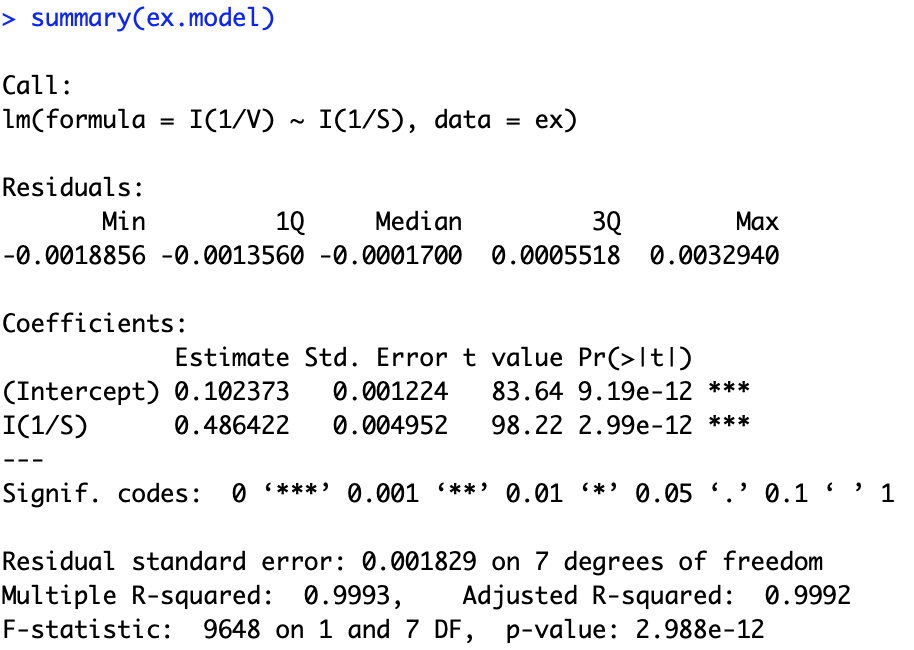
\includegraphics[width=0.5\textwidth]{output_ex_model.png}
	\caption{The output from the summary command. Several relevant outputs are displayed including the parameter estimates and their standard errors, with t-statistics and p-values for each, along with some information about the residuals, \(R^2\) value, and F-test information.}
	\end{figure}
		
\end{enumerate}

\end{document}